
\section{A Mechanistic Perspective on Weight Decay and Model Behavior}
\label{sec:explanation}

Prior work has shown that various factors can influence model plasticity, including the initialization state of model weights at the start of subsequent training, data representation (e.g., tokenization and categorical output representations), and model architecture (e.g., normalization layers)~\citep{ash2020shrinkandperturb, abagyan2025onetokenizer,lyle2023understanding}.
In Section~\ref{sec:exps}, we find that weight decay also shapes model plasticity.
In this section, we explore three mechanisms through which weight decay shapes model behavior: how weight decay shapes the pretrained model's internal representations, attention matrices, and the extent to which it overfits the pretraining data. We also discuss how each mechanism might explain why weight decay improves language model plasticity.





\begin{figure*}[t]
    \centering
    \begin{subfigure}[b]{0.24\textwidth}
        \centering
        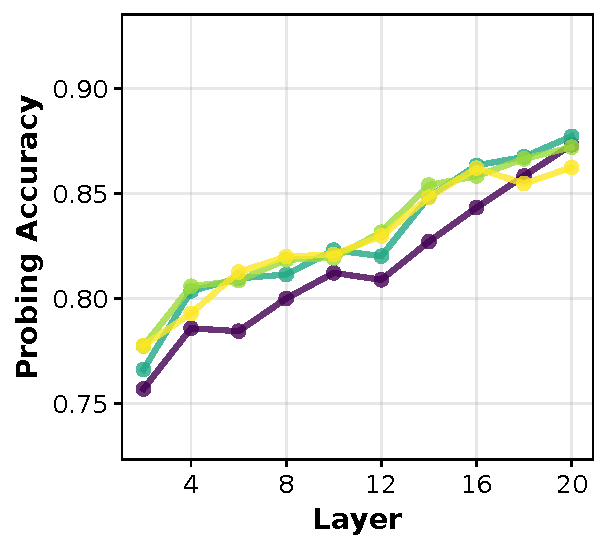
\includegraphics[width=\linewidth]{figs/a05_linear_probing/new/linear_probing_llama-0.5B-10BT.pdf}
        \caption{\llamazeropointfiveB{}}
    \end{subfigure}
    \hfill
    \begin{subfigure}[b]{0.24\textwidth}
        \centering
        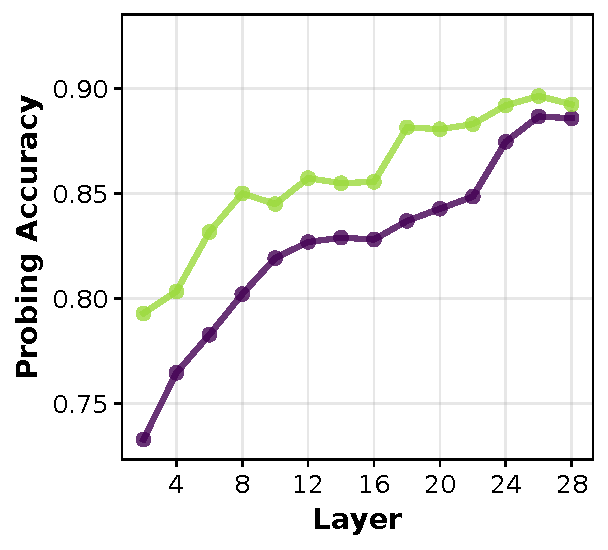
\includegraphics[width=\linewidth]{figs/a05_linear_probing/new/linear_probing_llama-4B-80BT.pdf}
        \caption{\llamafourB{}}
    \end{subfigure}
    \hfill
    \begin{subfigure}[b]{0.24\textwidth}
        \centering
        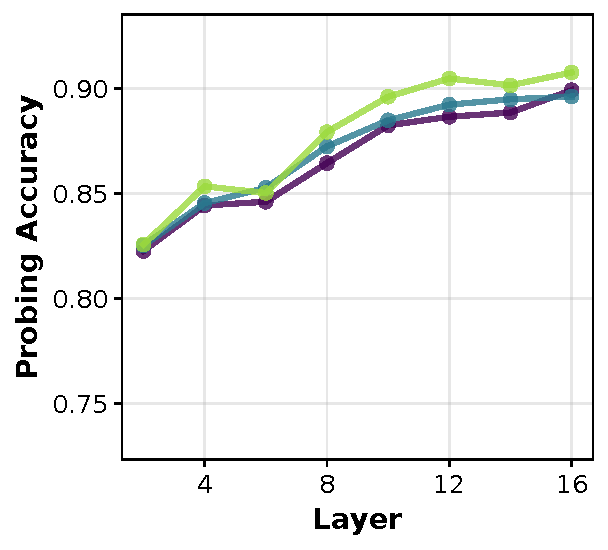
\includegraphics[width=\linewidth]{figs/a05_linear_probing/new/linear_probing_olmo-1B-30BT.pdf}
        \caption{\olmoonex{}}
    \end{subfigure}
    \hfill
    \begin{subfigure}[b]{0.24\textwidth}
        \centering
        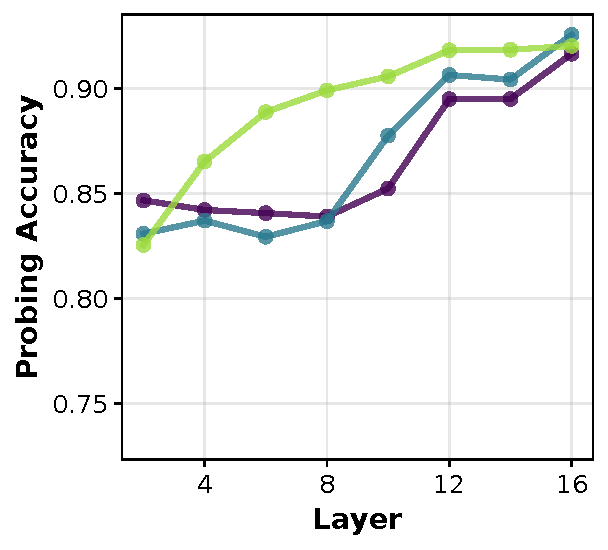
\includegraphics[width=\linewidth]{figs/a05_linear_probing/new/linear_probing_olmo-1B-210BT.pdf}
        \caption{\olmosevenx{}}
    \end{subfigure}$\,$\\[2pt]
    
\includegraphics[width=0.6\textwidth]{figs/a05_linear_probing/new/linear_probing_legend.pdf}
    \caption{{\bf Weight decay encourages linearly separated representations.} This figure depicts the accuracy of linear probes for sentiment and topic for models pretrained with different weight decay values. Stronger weight decay during pretraining results in higher linear probing accuracy, suggesting that weight decay promotes representations that are more linearly separable.}
    \label{fig:lin-probe}
\end{figure*}








\subsection{Weight decay encourages linearly separated representations}

Inspired by previous findings that weight decay leads to more structured representations in vision models~\citep{jacot2024neuralcollapse}, we investigate the effect of weight decay on the representations learned by pretrained language models. We pretrain models with varying weight decay, obtain the last-token embeddings for different types of text at a given model layer, and train a linear probe to classify these embeddings. We examine two tasks: classifying text based on sentiment (positive or negative movie reviews from the Stanford Sentiment Treebank dataset; \citet{socher2013sst}) or topic (four types of news articles from the AG News dataset; \citet{zhang2015agnews}). The average accuracy of these linear probes over the two tasks is shown in Figure~\ref{fig:lin-probe}. Accuracy for individual tasks are in Appendix~\ref{app:lin-probe}.

\begin{figure*}[t] 
    \centering
    \begin{subfigure}[b]{0.24\textwidth} 
        \centering
        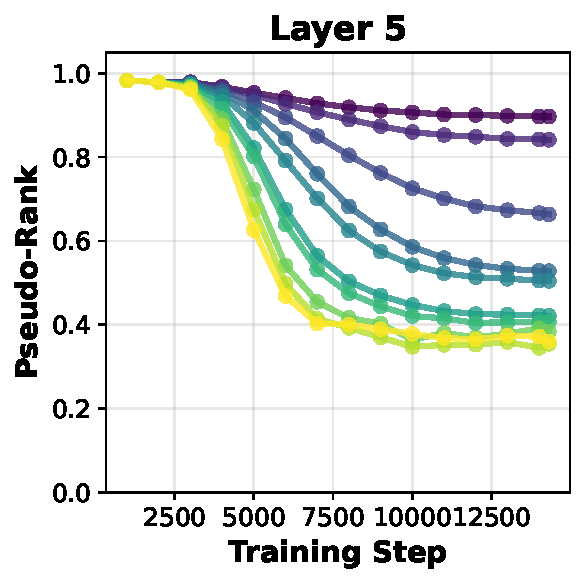
\includegraphics[width=\linewidth]{figs/rank_attn_matrices/layer5_qk.pdf} 
        \caption{Query-Key}
    \end{subfigure}
    \hfill
    \begin{subfigure}[b]{0.24\textwidth} 
        \centering
        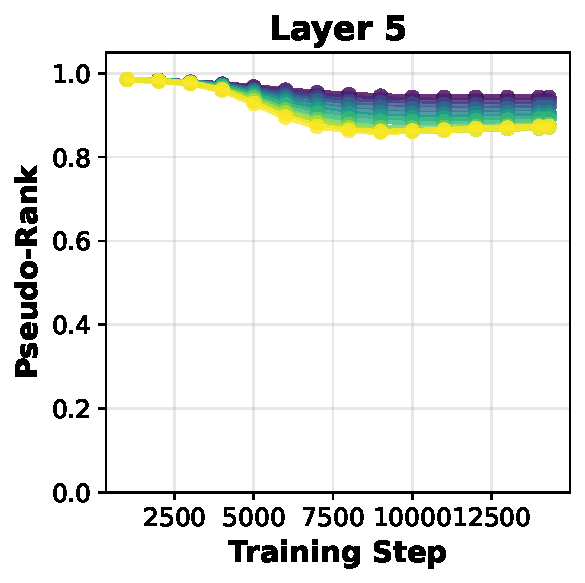
\includegraphics[width=\linewidth]{figs/rank_attn_matrices/layer5_vp.pdf} 
        \caption{Value-Projection}
    \end{subfigure}
    \hfill
    \begin{subfigure}[b]{0.24\textwidth} 
        \centering
        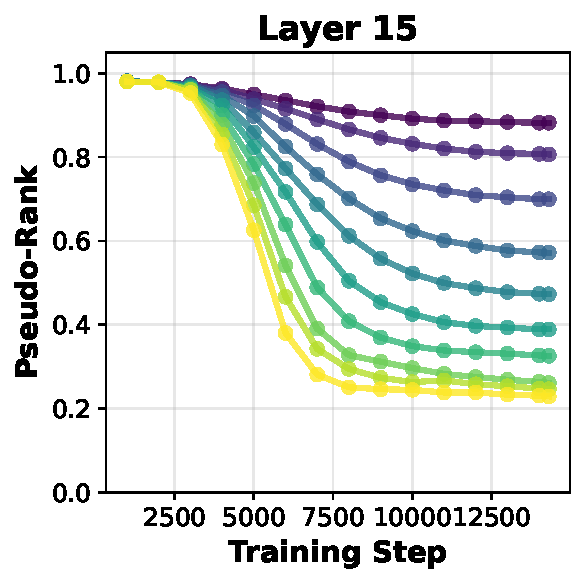
\includegraphics[width=\linewidth]{figs/rank_attn_matrices/layer15_qk.pdf} 
        \caption{Query-Key}
    \end{subfigure}
    \hfill
    \begin{subfigure}[b]{0.24\textwidth} 
        \centering
        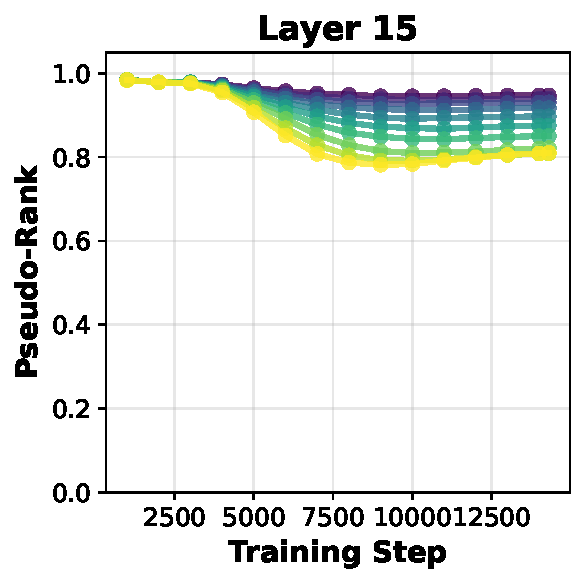
\includegraphics[width=\linewidth]{figs/rank_attn_matrices/layer15_vp.pdf} 
        \caption{Value-Projection}
    \end{subfigure}
    
\includegraphics[width=0.9\textwidth]{figs/rank_attn_matrices/olmo_legend.pdf}
    \caption{{\bf Weight decay reduces the rank of attention matrices.} This figure depicts the average pseudo-rank (Appendix \ref{app:pseudo_rank}) of the query-key ($W_{QK}$) and value projection ($W_{VP}$) matrices in layers 5 and 15 during the training of OLMo-2-1B models at 20 TPP. Stronger weight decay during pretraining leads to lower attention matrix ranks, suggesting that weight decay promotes a more compressed, lower-dimensional attention structure.}
    \label{fig:attention_rank_olmo}
\end{figure*}



We observe that when a given model is pretrained with higher weight decay, the accuracy of the linear probe trained on the model's representations tends to be higher at every layer of the model.
While this relationship is not perfectly monotonic (in some instances, a slightly higher weight decay can lead to a similar or slightly lower probing accuracy), it is generally consistent across weight decay values and model layers.
In addition, we observe this relationship  across model families, sizes, and training regimes (i.e., for all five model groups).
Thus, through these linear probing experiments, we find that representations from models pretrained with higher weight decay result in higher probing accuracies, indicating that these representations are more linearly separated and suggesting that models pretrained with higher weight decay form more structured internal representations.

The finding that weight decay shapes the representations of pretrained language models points to a potential explanation for why weight decay improves model plasticity (Section~\ref{subsec:exps-wd-plasticity}). Pretraining models with higher weight decay produces models with more structured representations, i.e., representations in which information is encoded in a more linearly accessible form. As a result, fine-tuning may focus on refining and aligning existing representations to the fine-tuning task rather than continuing to learn representations, effectively starting at a better initialization and leading to improved downstream performance. This hypothesis is consistent with previous findings that weight decay produces representations that are more transferable to downstream tasks in computer vision~\citep{lee2023rethinking}. It is further supported by the observation that the linear separability of model representations (probing accuracy) is strongly positively correlated with downstream model performance (Appendix Figure~\ref{fig:app-probeacc-vs-ftperf}).





\subsection{Weight decay reduces the rank of attention matrices}

Previous work by \citet{kobayashi2024wdlowrank} provides a theoretical argument that weight decay should reduce the rank of attention matrices. Recall that attention scores can be understood as a bilinear form $X^T W_{QK} X$ where $W_{QK}=W_K^T W_Q \in \mathbb{R}^{n_{embed} \times n_{embed}}$ is the product of the query and key matrices, and $X \in \mathbb{R}^{n_{embed} \times T}$ is the matrix of token embeddings (or hidden representations) for a sequence of length $T$. Now, the matrix $W_{QK}$ is naturally low-rank since its rank is at most $d_{head}$, which is usually significantly smaller than $n_{embed}$. \citet{kobayashi2024wdlowrank} argue that weight decay should further reduce the rank of $W_{QK}$, as well as of the value-projection matrix $W_{VP}=W_P W_V \in \mathbb{R}^{n_{embed} \times n_{embed}}$. 
\footnote{$W_{VP}$ is sometimes also denoted as $W_{VO}$ \citep{wang2025sharpness, wang2025muon}.} 
Concretely, they show that L2 regularization applied to the factored matrices $W_K$ and $W_Q$ becomes equivalent to nuclear norm regularization on their product $W_{QK}$, which is known to induce low rank by promoting sparsity in the singular values. While \citet{kobayashi2024wdlowrank} also provide empirical evidence on the Pile, their experiments were relatively small-scale from today’s perspective. We now revisit the impact of weight decay on the rank of attention in our more modern setup.


\textbf{Weight decay reduces the rank of attention, but default weight decay yields near full-rank matrices.} Figure \ref{fig:attention_rank_olmo} depicts the evolution of the pseudo-rank (Appendix \ref{app:pseudo_rank}) of the attention matrices during the training of the OLMo-2-1B-20x models. From Figure \ref{fig:attention_rank_olmo}, we observe that there is a monotonic relationship between the weight decay parameter and the rank of the attention matrices, where larger weight decay values reduce the rank of both $W_{QK}$ and $W_{VP}$. However, unlike what is observed in \citet{kobayashi2024wdlowrank}, we see that the default weight decay parameter of 0.1 yields near full-rank matrices.  This observation is further confirmed by Figure \ref{fig:attention_rank_training_time}, which shows that the attention matrices in the fully trained OLMo-2-1B model are nearly full-rank. 

\textbf{Attention matrices are differently affected by weight decay.} Another important observation from our experiments is that the rank of the matrix $W_{QK}$ seems to be significantly more sensitive to weight decay than $W_{VP}$. In our experiments, a weight decay of 1.0 reduces the rank of $W_{QK}$ by roughly a factor of 2, which is a common rank reduction observed in the literature on low-rank matrices. In contrast, the matrix $W_{VP}$ is still close to full-rank even for a large weight decay value of 1.0. These results are especially pronounced for Llama-2 models depicted in Figure \ref{fig:attention_rank_llama}, where the rank of $W_{VP}$ remains essentially stable up to a weight decay value of 1.0, after which the rank collapses—a transition that correlates with a significant drop in performance.

\textbf{Low-rank structure as a driver of adaptability.} The observation that increased weight decay leads to lower-rank attention matrices provides a potential explanation for why weight decay improves model plasticity. In machine learning literature, low-rank constraints are a canonical form of regularization that is often believed to encourage simpler, more robust hypotheses \citep{cai2010singular,oymak2019generalization,hu2022lora}. We conjecture that by encouraging $W_{QK}$ toward a lower-rank configuration, weight decay may prevent the model from overfitting to high-dimensional noise in the pretraining distribution.
Such a model may capture higher-level patterns that are more broadly applicable than details specific to the pretraining distribution, thereby enhancing the model’s ability to learn new data upon further training and improving downstream performance.



\subsection{Weight decay reduces overfitting on training data}


\begin{figure}[t] 
    \centering
    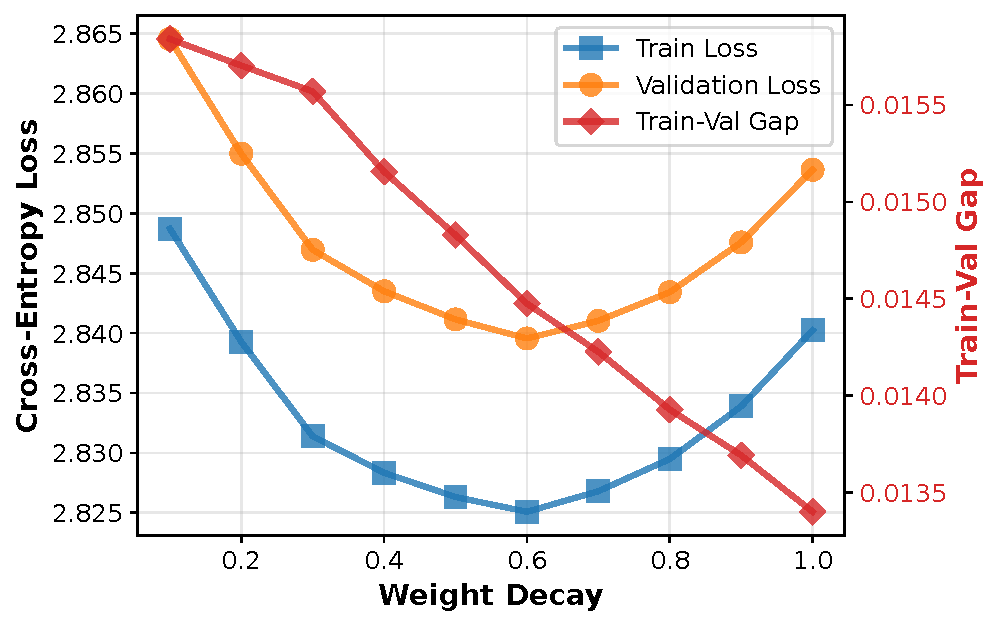
\includegraphics[width=0.9\linewidth]{figs/a04_val_loss/olmo_2_1b_1x_wd_ablation_train_val_loss.pdf}
    \caption{{\bf Weight decay reduces overfitting on training data.} This figure depicts the training loss, validation loss, and train-val gap (Equation~\ref{eq:train-val-gap}) for the \olmoonex{} models. As weight decay increases, the train-val gap decreases.} 
    \label{fig:wd_forgetting}
\end{figure}


Lastly, we explore how weight decay influences the extent to which the pretrained model overfits the pretraining data. Previous work has shown that weight decay can cause the forgetting of individual benchmark questions seen during pretraining \citep{bordt2025datacontam}. 
In the context of model plasticity, the ability to learn new information tends to be associated with the forgetting of prior data, a trade-off commonly referred to as the stability-plasticity dilemma~\citep{kirkpatrick2017overcoming,riemer2018learning,ibrahim2024simple,elsayed2024addressing}.
Building on these insights, we investigate how weight decay influences overfitting, which is closely related to the forgetting of training data, in pretrained models.



To measure the degree to which a pretrained model overfits the training data, we compute the difference between the loss on the validation data and that on the training data:
\begin{equation}
\label{eq:train-val-gap}
    \text{Train-Val Gap} = \text{Validation Loss} - \text{Training Loss}
\end{equation}
Here, the training loss is the average loss that the fully trained model encounters on the training data, which is distinct from the training loss curve or the final training loss value. A model that does not overfit the training data would theoretically have a train-val gap of zero. In practice, a larger train-val gap indicates a higher degree of overfitting on the training data, thus less forgetting of the training data.

Figure~\ref{fig:wd_forgetting} depicts the train-val gap for the OLMo-2 models trained at 20 TPP. We observe that the train-val gap decreases monotonically as the weight decay parameter is increased. This provides empirical evidence that models trained with larger weight decay values indeed overfit the training data less.


\begin{finding}
\textbf{Finding 3.} The pretraining weight decay hyperparameter has diverse mechanistic effects on model behavior. It encourages linearly separated representations, regularizes attention matrices, and reduces overfitting on the training data. 
\end{finding}















